\section{Results}
\label{results}

\subsection{Run~I Categorization}
The expected 95\% CL upper limit on the signal strength modifier has been
derived considering the Run~I event categories. Figure~\ref{combine:LimitsAsymptotic}
shows the limits derived using the Asimov data-set ({\bf blind}), including only the statistical
uncertainties.

%\begin{figure}[h!]
%    \centering
%     %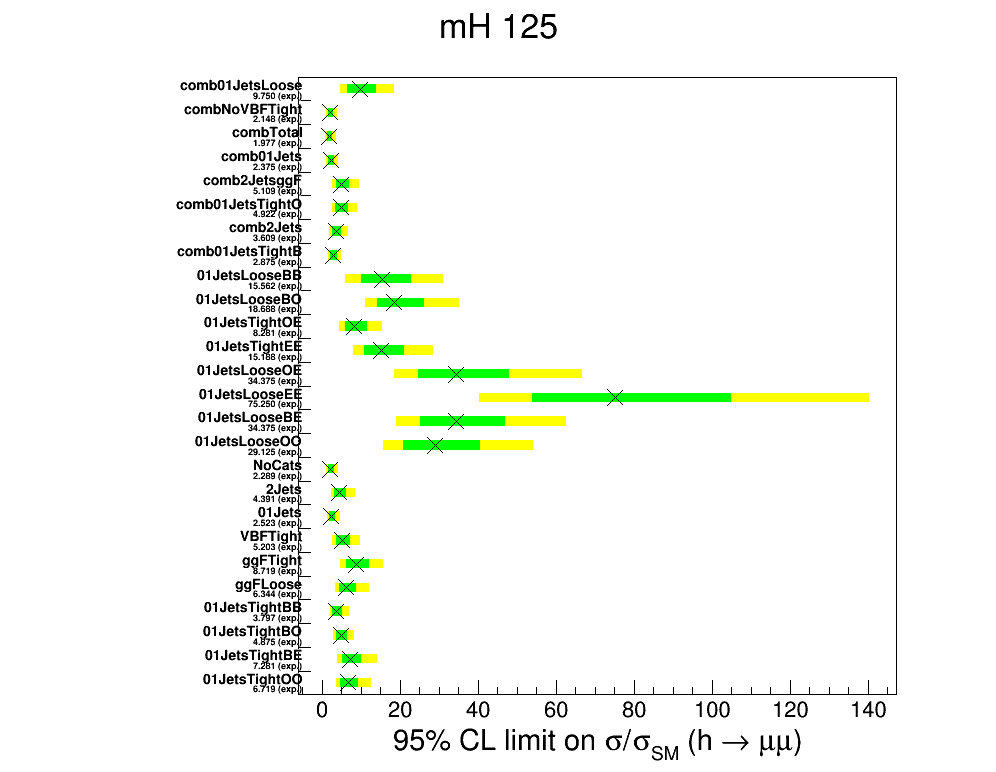
\includegraphics[width=0.45\textwidth]{figures/combine/limitsAsymptotic/baseline_110to160_p25GeV_NoNuis_Viktor/limitsByMass__125__TripleGaus.png}
%      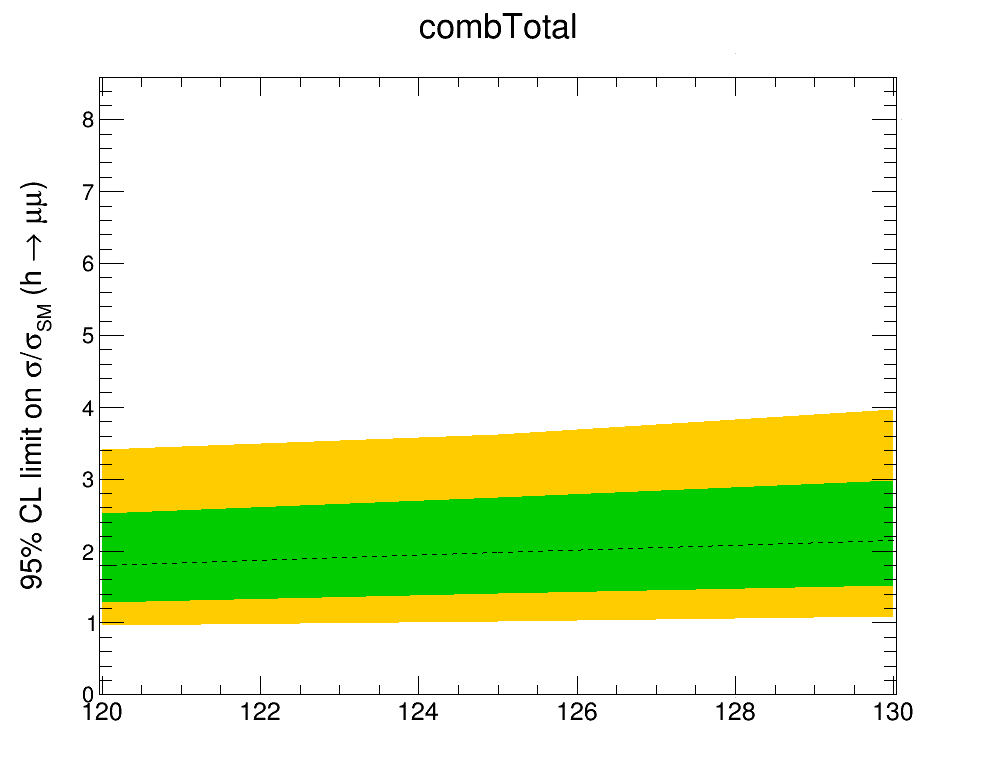
\includegraphics[width=0.618\textwidth]{figures/combine/limitsAsymptotic/baseline_110to160_p25GeV_NoNuis_Viktor/limitsByCategory__combTotal__TripleGaus.png}
%    \caption{95\% CL upper limit on the signal strength modifier. Limits are derived using the Asimov dataset ({\bf blind}) including only the statistical uncertainty.}
%    \label{results:limit}
%\end{figure}


%\clearpage
\subsection{Bdt Categorization}
Expected 95\% CL upper limit on the signal strength modifier have been derived
for the ``Bdt'' category based analysis and presented in
Fig.~\ref{results:limit}. The expected limits are derived using the Asimov
data-set ({\bf blind)}, using KF corrections and the following background
functions:  BWZredux ( cat 0, 2, 3, 7, 8, 9, 10, 11, 12), Bernstein
polynomial ( cat 1, 6), and SumExponential ( cat 4, 5). The expected
significance at $\mH=125\,\gev$ for SM Higgs boson is $0.85~\sigma$.

\begin{figure}[h!]
    \centering
    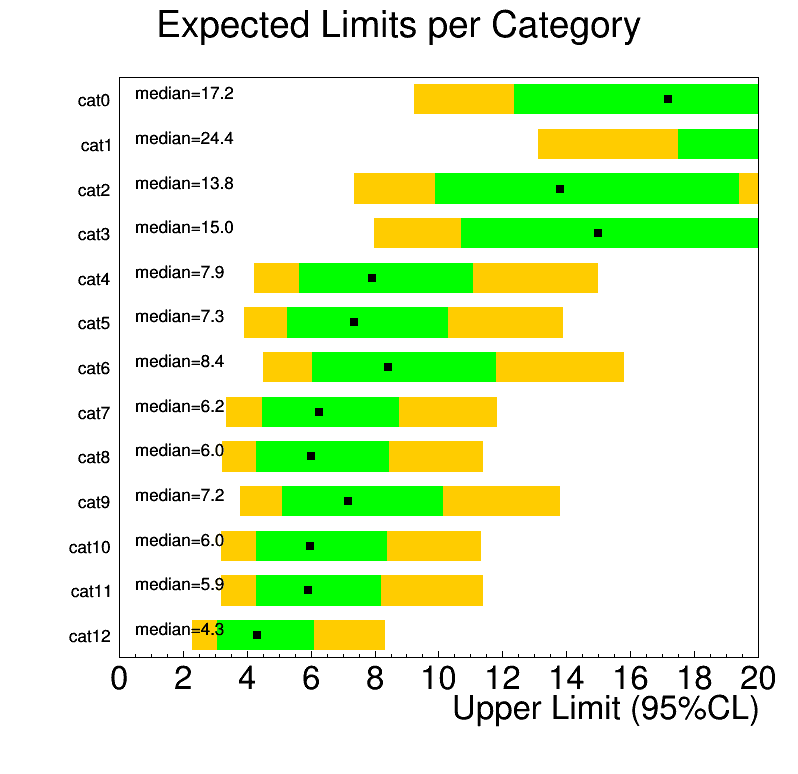
\includegraphics[width=0.681\textwidth]{figures/results/limitPerCategory}
    \caption{The 95\% CL upper limit on the signal strength modifier. Each
category is fitted independently. Limits are derived using the Asimov data-set
({\bf blind}). Systematic uncertainties are considered.}
    \label{results:limit_splitted}
\end{figure}

\begin{figure}[h!]
    \centering
    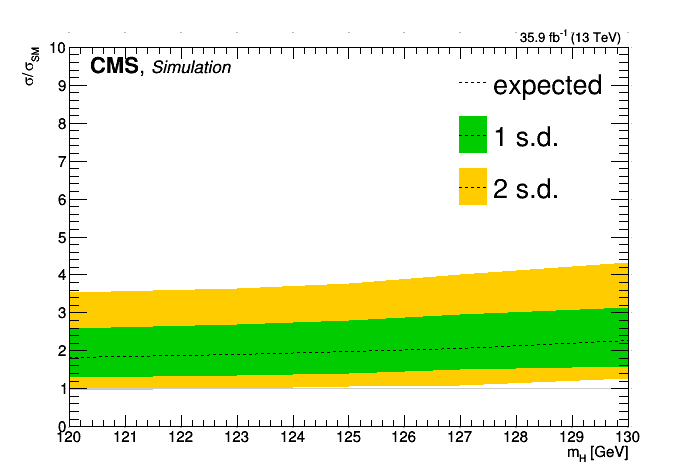
\includegraphics[width=0.681\textwidth]{figures/results/limit}
    \caption{The 95\% CL upper limit on the signal strength modifier. Limits
are derived using the Asimov data-set ({\bf blind}). Systematic uncertainties
are considered.}
    \label{results:limit}
\end{figure}


\begin{table}[h!]
    \centering
    \caption{95\% CL on the SM signal strength modifier}
    \begin{tabular}{lcccccc}
\hlinewd{1.2pt}
\multirow{2}{*}{$m_\textup{h}$ [GeV]} & \multicolumn{5}{c}{Expected Limits} & \multirow{2}{*}{Observed limit} \\
\cline{2-6}
& $-2\sigma$ & $-1\sigma$ & median  & $1\sigma$ & $2\sigma$ & \\
\hline
120 & 0.96 & 1.29 & 1.81 & 2.60 & 3.54 & - \\
123 & 1.01 & 1.35 & 1.90 & 2.69 & 3.64 & - \\
125 & 1.05 & 1.41 & 1.98 & 2.79 & 3.77 & - \\
127 & 1.10 & 1.50 & 2.07 & 2.96 & 4.00 & - \\
130 & 1.26 & 1.60 & 2.26 & 3.14 & 4.33 & - \\
\hlinewd{1.2pt}
\end{tabular}

\end{table}

Figure~\ref{results:mu} shows the best fit strength modifier,
$\hat{\mu}=1^{+2}_{-1}$.
\begin{figure}[h!]
    \centering
    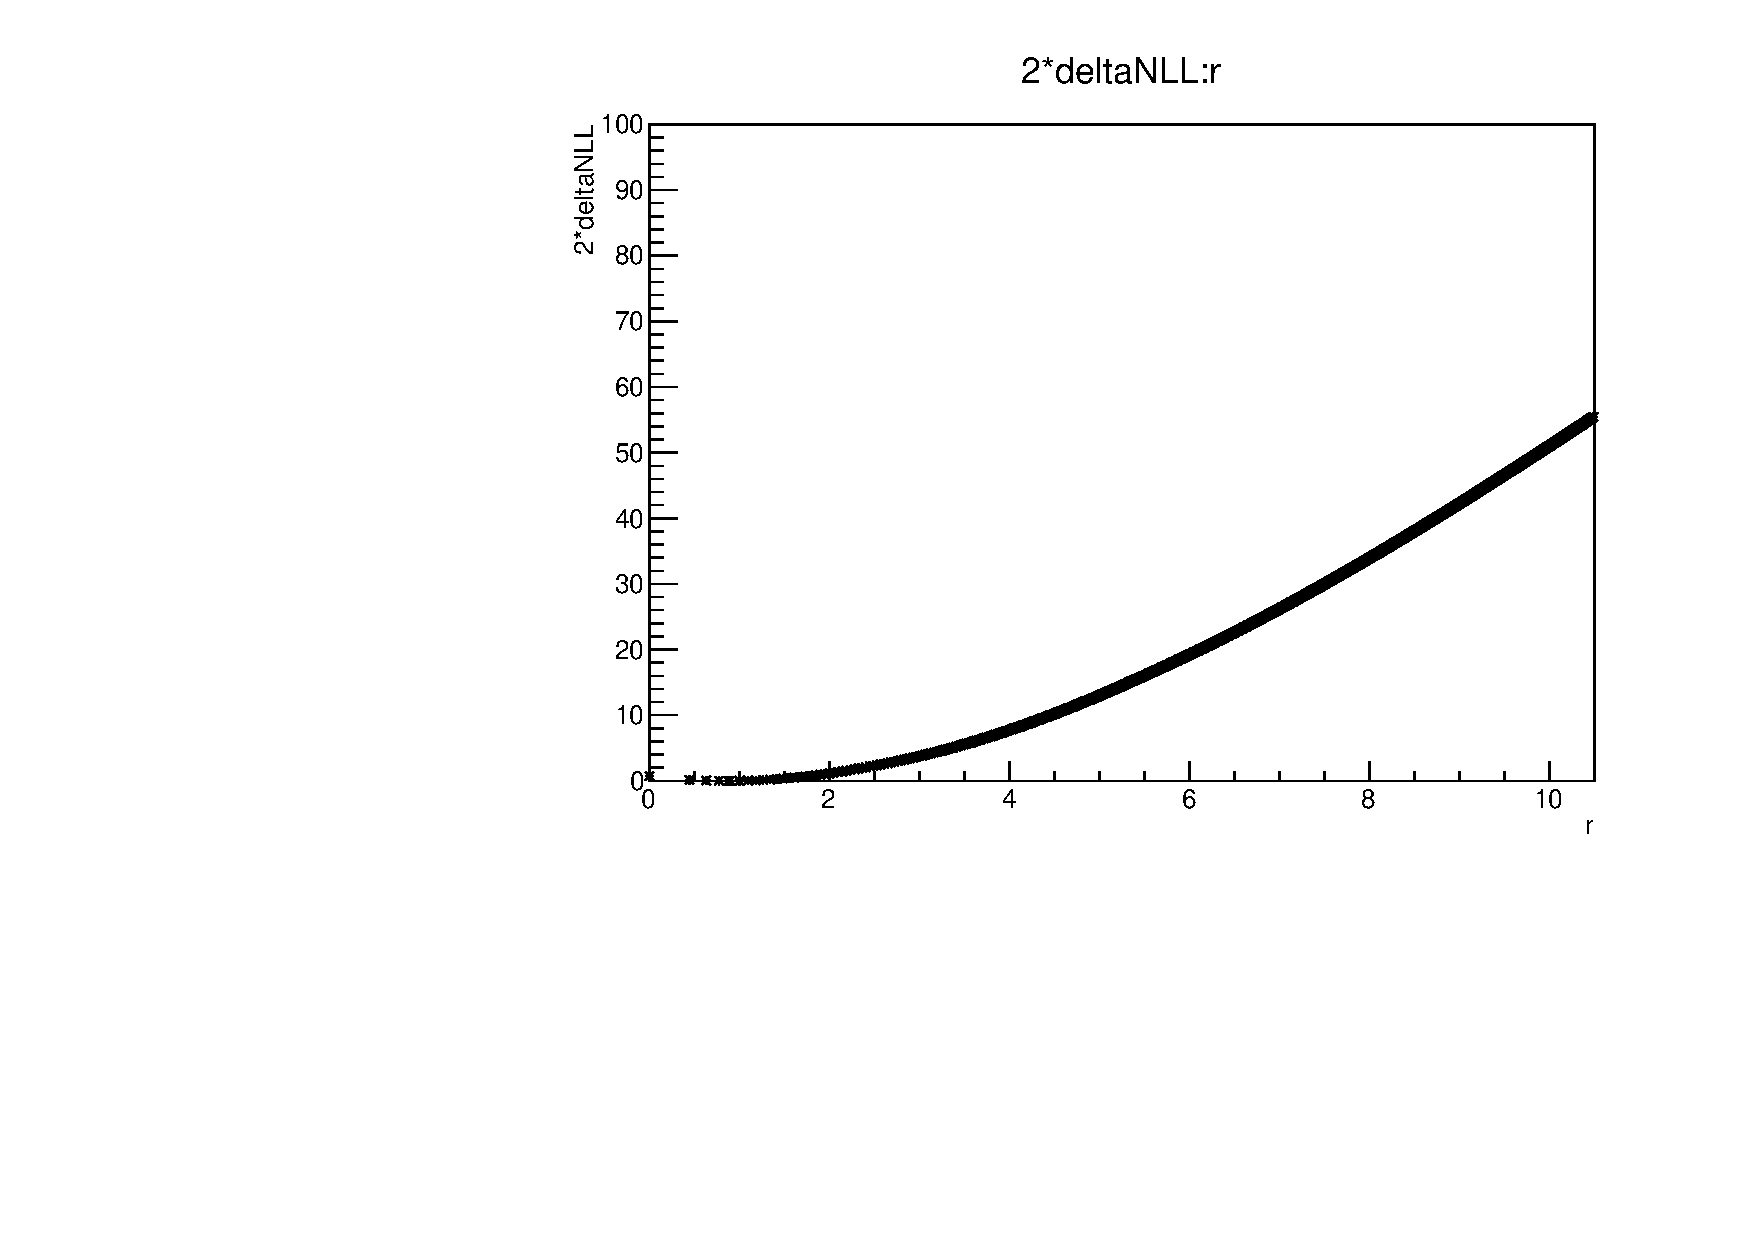
\includegraphics[width=0.681\textwidth]{figures/results/mu}
    \caption{The $2\Delta\log{\mathcal{L}}$ versus $\mu$. Scans are derived using the Asimov data-set ({\bf blind}).}
    \label{results:mu}
\end{figure}

Best fit of the strength modifier to the vector boson couplings (rV) and to
the fermion couplings (rF), floated independently, can be seen
in Fig.~\ref{results:rvrf}.
\begin{figure}[h!]
    \centering
    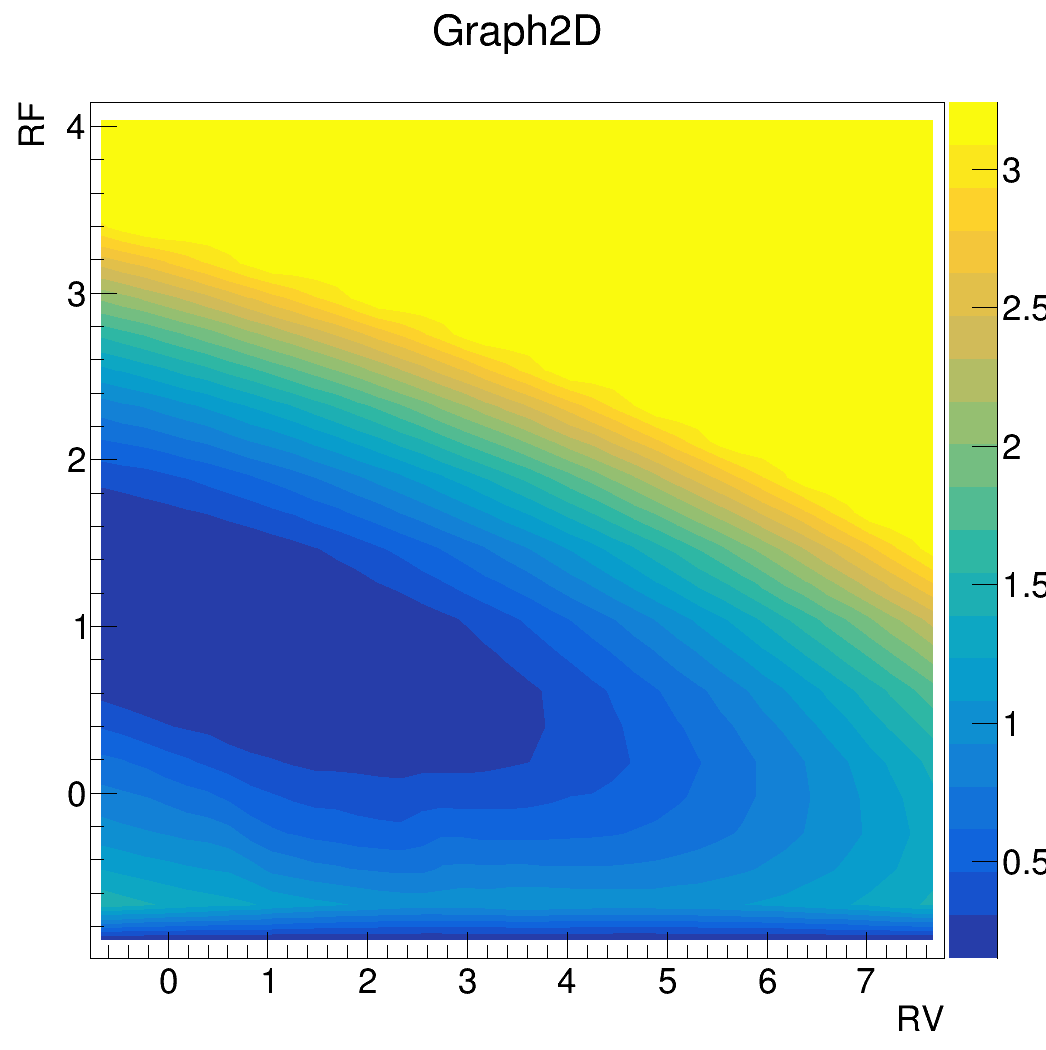
\includegraphics[width=0.681\textwidth]{figures/results/rV-rF}
    \caption{The $2\Delta\log{\mathcal{L}}$ versus rV-rF. Scans are derived
using the Asimov data-set ({\bf blind})}. Higgs boson mass is used as floating
parameter.
    \label{results:rvrf}
\end{figure}


%\clearpage
%\subsection{Combination}
%Combined limits are performed using $7$ and $8\,\tev$ datacards as sumbitted to svn.
%Details of these analyses can be found in Ref. cite-RunI-FIXME %% ~\cite{RunI}

%The following changes are performed:
%\begin{itemize}
%\item The signal yields have been multiplied by the value of $\sigma(\text{proc},\mH)_{YR4}/\sigma(\text{proc},\mH)_{YR3}$
%\item The signal yields have been multiplied by the value of $\mathcal{B}(\Htomm)_{YR4}/\mathcal{B}(\Htomm)_{YR3}$
%\end{itemize}

%Nuisances are all uncorrelated (conservative).

%\begin{figure}[h!]
%    \centering
%    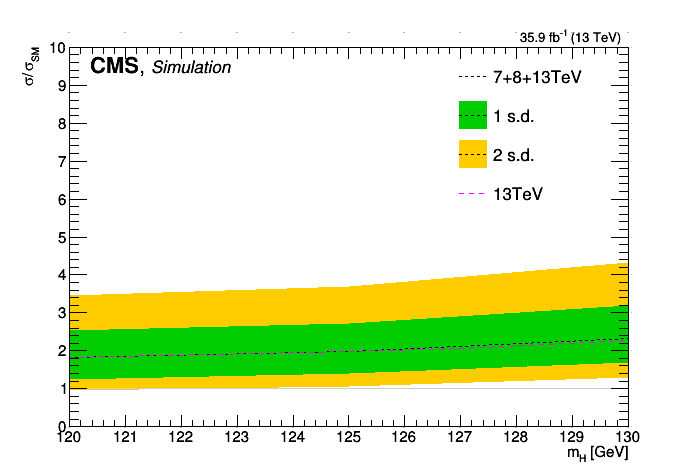
\includegraphics[width=0.681\textwidth]{figures/results/ExpLimitComb}
%    \caption{95\% CL upper limit on the signal strength modifier. Limits are derived using the Asimov dataset ({\bf blind})}
%    \label{results:comb_limit}
%\end{figure}

%\begin{table}[h!]
%    \centering
%    \caption{Combined Limits}
%    \begin{tabular}{lcccccc}
\hlinewd{1.2pt}
\multirow{2}{*}{$m_\textup{H}$ [GeV]} & \multicolumn{5}{c}{Expected Limits} & \multirow{2}{*}{Observed limit} \\
\cline{2-6}
& $-2\sigma$ & $-1\sigma$ & median  & $1\sigma$ & $2\sigma$ & \\
\hline
120 & 0.96 & 1.24 & 1.82 & 2.55 & 3.45 & - \\
125 & 1.05 & 1.41 & 1.98 & 2.73 & 3.69 & - \\
130 & 1.29 & 1.70 & 2.32 & 3.18 & 4.32 & - \\
\hlinewd{1.2pt}
\end{tabular}

%\end{table}
